\documentclass[conference]{IEEEtran}

% ====== Idioma y codificación ======
\usepackage[spanish]{babel}
\usepackage[utf8]{inputenc}
\usepackage[T1]{fontenc}

% ====== Paquetes útiles ======
\usepackage{graphicx}
\usepackage{booktabs}
\usepackage{tabularx}
\usepackage{hyperref}
\usepackage{csquotes}
\usepackage{url}
\usepackage{tikz}
\usetikzlibrary{positioning} % opcional, útil si luego quieres nodos relativos

% Para doble-columna en la parte inferior (figure*)
\usepackage{stfloats} % habilita [!b] en figure* con IEEEtran

% Para página en horizontal (rota la página completa en el PDF)
\usepackage{pdflscape}

% (Opcional) Nombres de autores y afiliación
\title{Historia de la Ingeniería de Software}
\author{
  \IEEEauthorblockN{Angel Luis Valdés Sánchez}
  \IEEEauthorblockA{Universidad Tecnológica de la Mixteca\\
  Huajuapan de León, Oaxaca, México\\
  \texttt{angelluis2605@gs.utm.mx}}
}

% (Opcional) Para mostrar números de página en IEEEtran conference:
\pagestyle{plain}

\begin{document}
\maketitle

\begin{abstract}
Este reporte presenta una síntesis histórica de la Ingeniería de Software desde los antecedentes previos a 1968 y la llamada \emph{crisis del software}, hasta los enfoques contemporáneos como Agile y DevOps. Se revisan hitos, modelos de proceso y estándares, destacando lecciones útiles para el desarrollo moderno y la enseñanza de la disciplina.
\end{abstract}

% \begin{IEEEkeywords}
% Historia de la Ingeniería de Software, crisis del software, Waterfall, Espiral, Agile, DevOps, CMMI, ISO/IEC, SWEBOK.
% \end{IEEEkeywords}

\section{Introducción}

La Ingeniería de Software surgió como respuesta a la creciente complejidad en el desarrollo de sistemas informáticos y a los problemas de calidad, costo y tiempo que marcaron las décadas de 1960 y 1970. La llamada \emph{crisis del software}, identificada en las conferencias de la OTAN de 1968 y 1969, puso de manifiesto que las prácticas informales y poco sistemáticas eran insuficientes para garantizar productos confiables \cite{booch2018history}. Desde entonces, la disciplina ha evolucionado de manera constante, incorporando nuevos modelos de proceso, estándares y metodologías que han transformado la manera en que se concibe, desarrolla y mantiene el software \cite{sommerville10e}.

El propósito de este trabajo es ofrecer una síntesis histórica de dicha evolución e identificar lecciones y patrones útiles para enfrentar retos actuales (entrega continua, automatización y aseguramiento de la calidad). El alcance abarca desde los antecedentes previos a la crisis del software hasta las tendencias contemporáneas, como el desarrollo ágil y la integración de prácticas DevOps, que reflejan la necesidad de mayor adaptabilidad y automatización en un mundo digitalizado \cite{pressman2019}.

La estructura del reporte es la siguiente: en la Sección II se presentan los antecedentes y la crisis del software; la Sección III aborda la evolución de los modelos de proceso, desde cascada hasta DevOps; la Sección IV discute la estandarización y profesionalización de la disciplina; y finalmente, la Sección V ofrece las conclusiones.


\section{Antecedentes, orígenes del término y crisis del software (1960--1970)}

Las primeras computadoras fueron humanos y, en su mayoría, mujeres dedicadas al cálculo manual de tablas astronómicas y matemáticas. Con la mecanización y la electrónica emergieron nuevas abstracciones (como el álgebra booleana, los lenguajes de alto nivel y las bibliotecas reutilizables) que elevaron el software a un nivel de artefacto independiente. Hitos como el IBM System/360 y la decisión de desacoplar el software del hardware consolidaron su valor económico y estimularon ecosistemas de colaboración y servicios \cite{booch2018history}.

El término \emph{ingeniería de software} suele atribuirse a la conferencia de la OTAN de 1968 o a la carta de Anthony Oettinger (1966), pero testimonios históricos indican que Margaret Hamilton ya lo empleaba entre 1963 y 1964 para distinguir su labor en los programas SAGE y Apollo del trabajo en hardware \cite{booch2018history}. En paralelo, la Guerra Fría impulsó sistemas críticos y distribuidos, como SAGE, que introdujeron innovaciones en interfaces humano--computadora, memoria y coordinación en tiempo real, elevando también los costos y riesgos asociados al software.

Durante las décadas de 1950 y 1960, el software comenzó a cobrar un papel cada vez más central en proyectos de defensa, investigación y administración. Sin embargo, la disciplina carecía de metodologías formales y se basaba en prácticas \textit{ad hoc}, fuertemente dependientes de la experiencia individual de los programadores. La creciente demanda de sistemas complejos puso en evidencia deficiencias significativas en calidad, plazos y costos. Ejemplos emblemáticos fueron el sistema operativo OS/360 de IBM, que demandó un esfuerzo técnico y económico mucho mayor al previsto \cite{brooks1975}, y el software del avión F-111 de la Fuerza Aérea de los Estados Unidos, cuyos problemas de integración derivaron en fallos críticos.

La magnitud del problema llevó a que en 1968 y 1969 se organizaran las conferencias de la OTAN sobre Ingeniería de Software, consideradas el punto de partida oficial de la disciplina. En dichos encuentros se acuñó el término de crisis del software para describir el fracaso recurrente de proyectos que no cumplían con los requisitos de funcionalidad, confiabilidad y entrega en tiempo. Los participantes, entre ellos Dijkstra y Naur, subrayaron la necesidad de aplicar principios de ingeniería al desarrollo de software, estableciendo las bases de lo que más tarde sería reconocido como Ingeniería de Software \cite{booch2018history}.

Las causas principales de esta crisis pueden resumirse en:
\begin{itemize}
    \item \textbf{Complejidad creciente:} sistemas más grandes y con múltiples dependencias, imposibles de manejar con técnicas de programación individuales.
    \item \textbf{Escalabilidad limitada:} dificultad para organizar y coordinar equipos de gran tamaño.
    \item \textbf{Calidad insuficiente:} software plagado de errores, costoso de mantener y con fallos críticos en producción.
    \item \textbf{Falta de procesos:} ausencia de estándares y metodologías sistemáticas para guiar el ciclo de vida del software.
\end{itemize}

La identificación de esta crisis marcó un punto de inflexión: el software dejó de considerarse un arte aislado para concebirse como un producto de ingeniería que requería procesos, estándares y metodologías. A partir de este momento, emergieron modelos de desarrollo como cascada y, posteriormente, espiral, que buscaban dar respuesta a las limitaciones detectadas en este periodo fundacional \cite{royce1970,boehm1988}.

\section{Evolución de modelos de proceso}

\subsection{Cascada y V-Model}
El modelo en cascada de Royce estructura el ciclo de vida en fases secuenciales con artefactos definidos (requisitos, diseño, implementación, verificación, mantenimiento). Sus supuestas claves, como requisitos estables y validación al final, aportaron control y trazabilidad, pero mostraron rigidez ante cambios y riesgos descubiertos tardíamente \cite{royce1970}. El V-Model reforzó la correspondencia entre construcción y prueba (aceptación, sistema, integración, unitarias), ganando tracción en dominios regulados (aeroespacial, médico, automotriz, defensa) \cite{sommerville10e}.

\subsection{Espiral y gestión del riesgo}
El modelo en espiral introdujo ciclos iterativos guiados por los \emph{objetivos, la evaluación de alternativas, el análisis de riesgos, el desarrollo y la validación}. Con prototipos tempranos y decisiones informadas por riesgo, mejoró el manejo de incertidumbre en sistemas de gran escala y de alto impacto, aunque exigió equipos con experiencia y disciplina para un análisis de riesgos efectivo \cite{boehm1988,pressman2019}.

\subsection{Modelos de madurez y calidad}
Durante los años 80 y 90 surgieron marcos de madurez y calidad (CMM/CMMI) enfocados en institucionalizar procesos y medición. En paralelo, se consolidó la normalización internacional del ciclo de vida, requisitos y calidad (ISO/IEC/IEEE 12207, 29148, 25010). Iniciativas como SWEBOK buscaron codificar el cuerpo de conocimiento de la disciplina y unificar terminología, prácticas y áreas de conocimiento \cite{booch2018history,swebok2014}.

\subsection{Agile y prácticas asociadas}
Con el auge de Internet y productos centrados en el usuario, métodos ágiles, como Scrum y XP, pasaron a ser el foco de atención tras el Manifiesto Ágil (2001). Su énfasis en iteración, entrega frecuente y retroalimentación acortó ciclos de validación y mejoró la alineación con el valor de negocio, a costa de requerir una fuerte disciplina técnica (pruebas automatizadas, diseño emergente) y una gestión rigurosa de la deuda técnica \cite{agile2001,sommerville10e}.

\subsection{DevOps y entrega continua}
Los DevOps, por su parte, integraron el desarrollo y las operaciones mediante la automatización de los \textit{pipelines} (CI/CD), la infraestructura como código y la observabilidad. Este enfoque redujo los tiempos de ciclo y mejoró la confiabilidad operativa, de forma tal que hoy es un pilar fundamental para sistemas distribuidos y arquitecturas basadas en servicios \cite{pressman2019,booch2018history}.

\section{Estandarización y profesionalización}

La estandarización formalizó lenguajes comunes y expectativas verificables entre actores técnicos y de negocio. ISO/IEC/IEEE 12207 estructuró procesos del ciclo de vida; ISO/IEC/IEEE 29148 definió prácticas de ingeniería de requisitos; ISO/IEC 25010 precisó modelos de calidad de producto y sistema \cite{sommerville10e}. Complementariamente, \emph{SWEBOK} (2004/2014) sistematizó el cuerpo de conocimiento en áreas (requisitos, diseño, construcción, pruebas, mantenimiento, gestión, procesos, herramientas y métodos), contribuyendo a la profesionalización y a la educación de la disciplina \cite{swebok2014,booch2018history}.

\section{Conclusiones}

La evolución de la Ingeniería de Software muestra un patrón de respuestas progresivas a las limitaciones de los enfoques anteriores. La predictibilidad documental del modelo en cascada fue complementada por el control explícito del riesgo en el espiral; la madurez de procesos aportó repetibilidad y medición; la agilidad aceleró el aprendizaje con el usuario mediante entregas frecuentes; y DevOps cerró el ciclo con la automatización operativa y la integración continua. Estos avances no deben entenderse como sustituciones, sino como capas que se superponen y enriquecen el cuerpo de prácticas de la disciplina.

A pesar de los logros alcanzados, persiste el reto de equilibrar flexibilidad con control, sostener la calidad mediante evidencia objetiva (pruebas, métricas) y gestionar de manera efectiva la deuda técnica acumulada a lo largo del ciclo de vida. Los escenarios actuales introducen además nuevos desafíos, como la integración de inteligencia artificial en actividades de especificación y pruebas, la necesidad de verificación continua en entornos regulados y la creciente presión por garantizar seguridad y confiabilidad en sistemas distribuidos y críticos.

La trayectoria histórica sugiere que la Ingeniería de Software continuará transformándose al ritmo de las tecnologías y las demandas sociales, pero mantendrá como núcleo inalterable la búsqueda de confiabilidad, calidad y valor entregado al usuario.


% ====== Bibliografía (BibTeX + IEEEtran) ======
\bibliographystyle{IEEEtran}
\bibliography{refs}


% \clearpage
% \begin{landscape} % página horizontal
% \begin{figure*}[!b]
%   \centering
%   % Usa la versión que tengas disponible:
%   % \includegraphics[width=\textwidth]{fig/timeline_preview.pdf}
%   \includegraphics[width=\textwidth]{timeline_preview.png}
%   \caption{Línea de tiempo de hitos en la evolución de la Ingeniería de Software.}
%   \label{fig:timeline}
% \end{figure*}
% \end{landscape}
% \clearpage

\end{document}
